\chapter{グラフ探索 - Graph traversal}


この章では、深さ優先探索(DFS)と幅優先探索(BFS)という2つの基本的なグラフアルゴリズムについて説明します。
どちらのアルゴリズムもグラフの開始ノードが与えられ、その開始ノードからすべての到達可能なノードを訪問し、
両者はこの訪問順序が異なります。

\section{深さ優先探索 - Depth-first search}

\index{depth-first search}

\key{深さ優先探索(Depth-first search)} (DFS)は直線的なグラフ探索技法です。
開始ノードからエッジを使用して到達可能な他のすべてのノードに進みます。
深さ優先探索は、新しいノードがある限り常にグラフ内の下側に辿ります。
行き止まりになったら、前のノードに戻りグラフの他の部分の探索を開始します。
このアルゴリズムは、訪問したノードを記録しておき各ノードを一度だけ処理するようにします。

\subsubsection*{例}
次のグラフを深さ優先探索で処理する方法を考えます。

\begin{center}
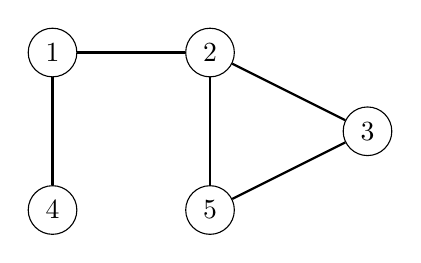
\begin{tikzpicture}
\node[draw, circle] (1) at (1,5) {$1$};
\node[draw, circle] (2) at (3,5) {$2$};
\node[draw, circle] (3) at (5,4) {$3$};
\node[draw, circle] (4) at (1,3) {$4$};
\node[draw, circle] (5) at (3,3) {$5$};

\path[draw,thick,-] (1) -- (2);
\path[draw,thick,-] (2) -- (3);
\path[draw,thick,-] (1) -- (4);
\path[draw,thick,-] (3) -- (5);
\path[draw,thick,-] (2) -- (5);
\end{tikzpicture}
\end{center}
グラフのどのノードから検索を始めても良いですが、ここではノード1から検索を始めます。

まず、ノード2を探索します。
\begin{center}
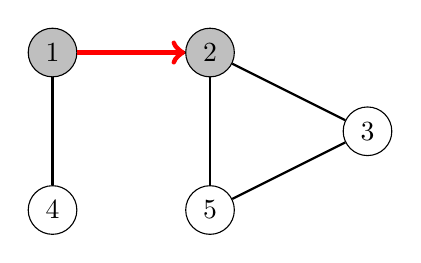
\begin{tikzpicture}
\node[draw, circle,fill=lightgray] (1) at (1,5) {$1$};
\node[draw, circle,fill=lightgray] (2) at (3,5) {$2$};
\node[draw, circle] (3) at (5,4) {$3$};
\node[draw, circle] (4) at (1,3) {$4$};
\node[draw, circle] (5) at (3,3) {$5$};

\path[draw,thick,-] (1) -- (2);
\path[draw,thick,-] (2) -- (3);
\path[draw,thick,-] (1) -- (4);
\path[draw,thick,-] (3) -- (5);
\path[draw,thick,-] (2) -- (5);

\path[draw=red,thick,->,line width=2pt] (1) -- (2);
\end{tikzpicture}
\end{center}

そして、3,5と訪問したとします。
\begin{center}
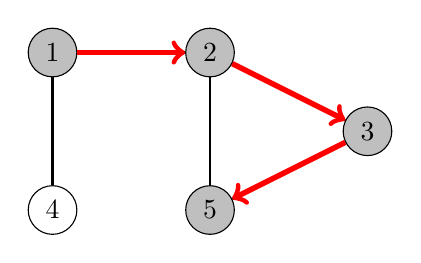
\begin{tikzpicture}
\node[draw, circle,fill=lightgray] (1) at (1,5) {$1$};
\node[draw, circle,fill=lightgray] (2) at (3,5) {$2$};
\node[draw, circle,fill=lightgray] (3) at (5,4) {$3$};
\node[draw, circle] (4) at (1,3) {$4$};
\node[draw, circle,fill=lightgray] (5) at (3,3) {$5$};

\path[draw,thick,-] (1) -- (2);
\path[draw,thick,-] (2) -- (3);
\path[draw,thick,-] (1) -- (4);
\path[draw,thick,-] (3) -- (5);
\path[draw,thick,-] (2) -- (5);

\path[draw=red,thick,->,line width=2pt] (1) -- (2);
\path[draw=red,thick,->,line width=2pt] (2) -- (3);
\path[draw=red,thick,->,line width=2pt] (3) -- (5);
\end{tikzpicture}
\end{center}
ノード5の隣接ノードは2と3ですが、
すでにその両方を訪れているので、前のノードに戻ります。
また、ノード3と2の隣接ノードは全て訪問済みなので、
次はノード1からノード4へ移動することになります。
\begin{center}
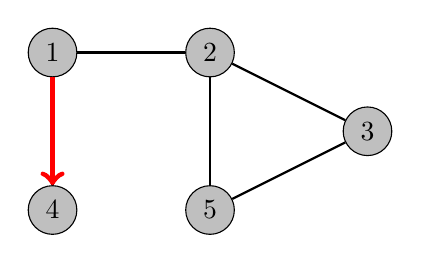
\begin{tikzpicture}
\node[draw, circle,fill=lightgray] (1) at (1,5) {$1$};
\node[draw, circle,fill=lightgray] (2) at (3,5) {$2$};
\node[draw, circle,fill=lightgray] (3) at (5,4) {$3$};
\node[draw, circle,fill=lightgray] (4) at (1,3) {$4$};
\node[draw, circle,fill=lightgray] (5) at (3,3) {$5$};

\path[draw,thick,-] (1) -- (2);
\path[draw,thick,-] (2) -- (3);
\path[draw,thick,-] (1) -- (4);
\path[draw,thick,-] (3) -- (5);
\path[draw,thick,-] (2) -- (5);

\path[draw=red,thick,->,line width=2pt] (1) -- (4);
\end{tikzpicture}
\end{center}

これですべてのノードを訪問したので探索は終了します。

深さ優先探索の時間計算量は $O(n + m)$ ($n$ はノードの数、$m$ はエッジの数)です。
なぜなら全てのノードと辺が1回ずつ辿るからです。

\subsubsection*{DFSの実装}

深さ優先探索は再帰を使って簡単に実装できます。
次の関数  \texttt{dfs}  は,引数に与えられたノードから深さ優先探索を開始します。
この関数は,グラフを隣接リストとして参照します。
\begin{lstlisting}
vector<int> adj[N];
\end{lstlisting}
また、次の配列を訪問済みのノードの情報として利用します。
\begin{lstlisting}
bool visited[N];
\end{lstlisting}
訪問済みリストの値は最初全て\texttt{false}です。
そして、$s$でこの関数が呼ばれると\texttt{visited}[$s$] は \texttt{true}になります。
この関数は以下のように実装できます。
\begin{lstlisting}
void dfs(int s) {
    if (visited[s]) return;
    visited[s] = true;
    // process node s
    for (auto u: adj[s]) {
        dfs(u);
    }
}
\end{lstlisting}

\section{幅優先探索 - Breadth-first search}

\index{breadth-first search}

\key{幅優先探索 - Breadth-first search} (BFS)は、開始ノードからの距離順が小さい順にノードを訪問していきます。
つまり、BFSを用いると始点ノードから他のすべてのノードまでの距離を計算することができます(訳註: これはDFSでも可能です)。
ただし、BFSは深さ優先探索よりも実装が複雑になります。
BFSはノードを深さごとに見ていきます。まず、開始ノードからの距離が1であるノードを探索し、次に距離が2であるノードを探索し、
というようにすべてのノードが訪問されるまで続けられます。

\subsubsection*{例}
次のようなグラフに対して、幅優先探索がどのように処理されるかを考えてみよう。

\begin{center}
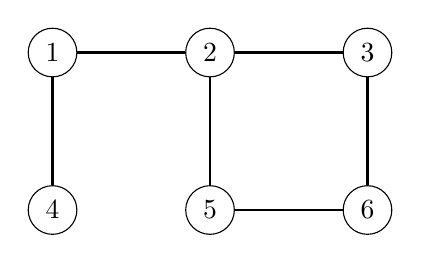
\begin{tikzpicture}
\node[draw, circle] (1) at (1,5) {$1$};
\node[draw, circle] (2) at (3,5) {$2$};
\node[draw, circle] (3) at (5,5) {$3$};
\node[draw, circle] (4) at (1,3) {$4$};
\node[draw, circle] (5) at (3,3) {$5$};
\node[draw, circle] (6) at (5,3) {$6$};

\path[draw,thick,-] (1) -- (2);
\path[draw,thick,-] (2) -- (3);
\path[draw,thick,-] (1) -- (4);
\path[draw,thick,-] (3) -- (6);
\path[draw,thick,-] (2) -- (5);
\path[draw,thick,-] (5) -- (6);
\end{tikzpicture}
\end{center}

ノード1から探索を開始したとします。最初に、ノード1から直接つながっている1つの辺で到達可能なすべてのノードを探索します。
\begin{center}
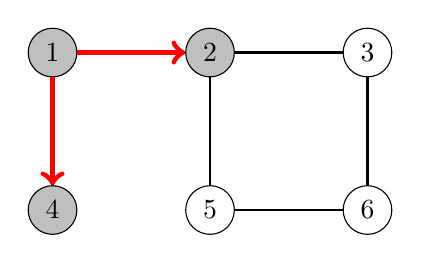
\begin{tikzpicture}
\node[draw, circle,fill=lightgray] (1) at (1,5) {$1$};
\node[draw, circle,fill=lightgray] (2) at (3,5) {$2$};
\node[draw, circle] (3) at (5,5) {$3$};
\node[draw, circle,fill=lightgray] (4) at (1,3) {$4$};
\node[draw, circle] (5) at (3,3) {$5$};
\node[draw, circle] (6) at (5,3) {$6$};

\path[draw,thick,-] (1) -- (2);
\path[draw,thick,-] (2) -- (3);
\path[draw,thick,-] (1) -- (4);
\path[draw,thick,-] (3) -- (6);
\path[draw,thick,-] (2) -- (5);
\path[draw,thick,-] (5) -- (6);

\path[draw,thick,-] (1) -- (2);
\path[draw,thick,-] (2) -- (3);
\path[draw,thick,-] (1) -- (4);
\path[draw,thick,-] (2) -- (5);

\path[draw=red,thick,->,line width=2pt] (1) -- (2);
\path[draw=red,thick,->,line width=2pt] (1) -- (4);
\end{tikzpicture}
\end{center}
その後、ノード3、ノード5を探索します。

\begin{center}
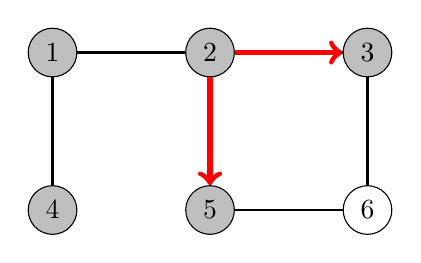
\begin{tikzpicture}
\node[draw, circle,fill=lightgray] (1) at (1,5) {$1$};
\node[draw, circle,fill=lightgray] (2) at (3,5) {$2$};
\node[draw, circle,fill=lightgray] (3) at (5,5) {$3$};
\node[draw, circle,fill=lightgray] (4) at (1,3) {$4$};
\node[draw, circle,fill=lightgray] (5) at (3,3) {$5$};
\node[draw, circle] (6) at (5,3) {$6$};

\path[draw,thick,-] (1) -- (2);
\path[draw,thick,-] (2) -- (3);
\path[draw,thick,-] (1) -- (4);
\path[draw,thick,-] (3) -- (6);
\path[draw,thick,-] (2) -- (5);
\path[draw,thick,-] (5) -- (6);

\path[draw,thick,-] (1) -- (2);
\path[draw,thick,-] (2) -- (3);
\path[draw,thick,-] (1) -- (4);
\path[draw,thick,-] (2) -- (5);

\path[draw=red,thick,->,line width=2pt] (2) -- (3);
\path[draw=red,thick,->,line width=2pt] (2) -- (5);
\end{tikzpicture}
\end{center}
最後に、ノード6が探索されます。

\begin{center}
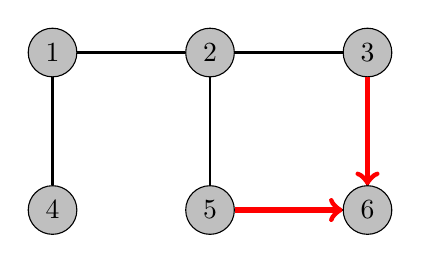
\begin{tikzpicture}
\node[draw, circle,fill=lightgray] (1) at (1,5) {$1$};
\node[draw, circle,fill=lightgray] (2) at (3,5) {$2$};
\node[draw, circle,fill=lightgray] (3) at (5,5) {$3$};
\node[draw, circle,fill=lightgray] (4) at (1,3) {$4$};
\node[draw, circle,fill=lightgray] (5) at (3,3) {$5$};
\node[draw, circle,fill=lightgray] (6) at (5,3) {$6$};

\path[draw,thick,-] (1) -- (2);
\path[draw,thick,-] (2) -- (3);
\path[draw,thick,-] (1) -- (4);
\path[draw,thick,-] (3) -- (6);
\path[draw,thick,-] (2) -- (5);
\path[draw,thick,-] (5) -- (6);

\path[draw,thick,-] (1) -- (2);
\path[draw,thick,-] (2) -- (3);
\path[draw,thick,-] (1) -- (4);
\path[draw,thick,-] (2) -- (5);

\path[draw=red,thick,->,line width=2pt] (3) -- (6);
\path[draw=red,thick,->,line width=2pt] (5) -- (6);
\end{tikzpicture}
\end{center}

開始ノードからグラフの全ノードまでの距離を以下のように計算できました。

\begin{tabular}{ll}
\\
node & distance \\
\hline
1 & 0 \\
2 & 1 \\
3 & 2 \\
4 & 1 \\
5 & 2 \\
6 & 3 \\
\\
\end{tabular}


BFSもDFSと同様に$O(n+m)$の計算量で実行できます。先ほどと同様に$n$が辺の数、
$m$が頂点とします。

\subsubsection*{実装}

BFSは今探索しているノードとは異なる部分のノードを訪問するため、DFSよりも実装が少し複雑になります。
最もシンプルなアプローチは探索するノードのキューを持ち、各ステップではキュー内の最初のノードを処理します。

以下のコードはグラフが隣接リストとして格納され、以下の変数を保持することを想定しています。

\begin{lstlisting}
queue<int> q;
bool visited[N];
int distance[N];
\end{lstlisting}

キュー\texttt{q} には処理すべきノードが距離の昇順に並んでいます。
新しいノードは常にキューの末尾に追加されて待ち行列の先頭にあるノードが次に処理されるノードとなる。
配列\texttt{visited}は訪問済みのノードであるかを持ち、
配列\texttt{distance}は開始ノードからグラフの全ノードまでの距離を持ちます。

ノード\texttt{x} から始まる探索は,以下のように実装できます。
\begin{lstlisting}
visited[x] = true;
distance[x] = 0;
q.push(x);
while (!q.empty()) {
    int s = q.front(); q.pop();
    // process node s
    for (auto u : adj[s]) {
        if (visited[u]) continue;
        visited[u] = true;
        distance[u] = distance[s]+1;
        q.push(u);
    }
}
\end{lstlisting}


\section{応用 - Applications}


グラフの探索アルゴリズムを用いると、いくつかのグラフの特性を確認することができます。
多くのケースでDFS,BFSの両方を用いることができますが、実装が簡易性からDFSを選択することが多いでしょう。
以下の応用例では、グラフは無向であると仮定する。

\subsubsection{連結性チェック - Connectivity check}

\index{connected graph}

グラフの任意の2つのノード間にパスが存在するとき、グラフは連結していると言えます。
つまり任意のノードから出発して、他のすべてのノードに到達できるかどうかを調べれば、グラフが連結されているかどうかを調べることができます。

例えば次のようなグラフを考えます。
\begin{center}
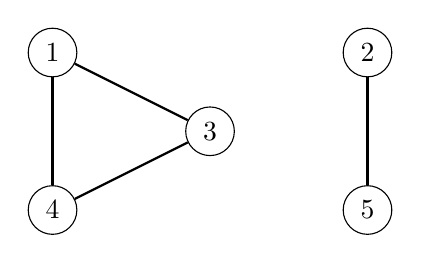
\begin{tikzpicture}
\node[draw, circle] (2) at (7,5) {$2$};
\node[draw, circle] (1) at (3,5) {$1$};
\node[draw, circle] (3) at (5,4) {$3$};
\node[draw, circle] (5) at (7,3) {$5$};
\node[draw, circle] (4) at (3,3) {$4$};

\path[draw,thick,-] (1) -- (3);
\path[draw,thick,-] (1) -- (4);
\path[draw,thick,-] (3) -- (4);
\path[draw,thick,-] (2) -- (5);
\end{tikzpicture}
\end{center}

DFSをノード1から実行します。
\begin{center}
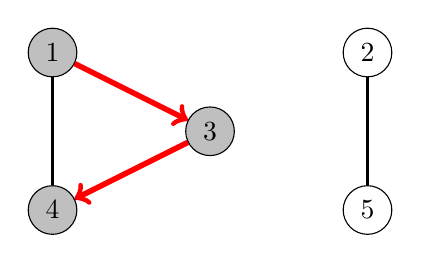
\begin{tikzpicture}
\node[draw, circle] (2) at (7,5) {$2$};
\node[draw, circle,fill=lightgray] (1) at (3,5) {$1$};
\node[draw, circle,fill=lightgray] (3) at (5,4) {$3$};
\node[draw, circle] (5) at (7,3) {$5$};
\node[draw, circle,fill=lightgray] (4) at (3,3) {$4$};

\path[draw,thick,-] (1) -- (3);
\path[draw,thick,-] (1) -- (4);
\path[draw,thick,-] (3) -- (4);
\path[draw,thick,-] (2) -- (5);

\path[draw=red,thick,->,line width=2pt] (1) -- (3);
\path[draw=red,thick,->,line width=2pt] (3) -- (4);

\end{tikzpicture}
\end{center}

この結果、すべてのノードが訪問されなかったので、このグラフは連結されていないと結論づけられます。
このあと、探索されていないノードからさらに新しい深さ優先探索を開始することにより、グラフのすべての連結成分を見つけることもできます。


\subsubsection{閉路の検出 - Finding cycles}

\index{cycle}

あるノードの探索中に、(現在のパスの前のノード以外の)その隣接ノードがすでに訪問されている場合、グラフはサイクルを含んでいることになります。

これも例で示します。
\begin{center}
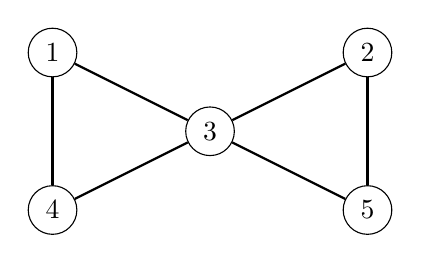
\begin{tikzpicture}
\node[draw, circle] (2) at (7,5) {$2$};
\node[draw, circle] (1) at (3,5) {$1$};
\node[draw, circle] (3) at (5,4) {$3$};
\node[draw, circle] (5) at (7,3) {$5$};
\node[draw, circle] (4) at (3,3) {$4$};

\path[draw,thick,-] (1) -- (3);
\path[draw,thick,-] (1) -- (4);
\path[draw,thick,-] (3) -- (4);
\path[draw,thick,-] (2) -- (5);
\path[draw,thick,-] (2) -- (3);
\path[draw,thick,-] (3) -- (5);
\end{tikzpicture}
\end{center}

これには2つの閉路が含まれます。例えばこの1つを見つけるのは以下のように行われます。
\begin{center}
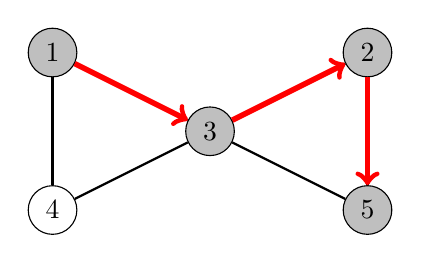
\begin{tikzpicture}
\node[draw, circle,fill=lightgray] (2) at (7,5) {$2$};
\node[draw, circle,fill=lightgray] (1) at (3,5) {$1$};
\node[draw, circle,fill=lightgray] (3) at (5,4) {$3$};
\node[draw, circle,fill=lightgray] (5) at (7,3) {$5$};
\node[draw, circle] (4) at (3,3) {$4$};

\path[draw,thick,-] (1) -- (3);
\path[draw,thick,-] (1) -- (4);
\path[draw,thick,-] (3) -- (4);
\path[draw,thick,-] (2) -- (5);
\path[draw,thick,-] (2) -- (3);
\path[draw,thick,-] (3) -- (5);

\path[draw=red,thick,->,line width=2pt] (1) -- (3);
\path[draw=red,thick,->,line width=2pt] (3) -- (2);
\path[draw=red,thick,->,line width=2pt] (2) -- (5);

\end{tikzpicture}
\end{center}


ノード2からノード5に移動した後、ノード5の隣接ノード3はすでに訪問済みであるとわかります。
したがって,このグラフには,例えば
$3 \rightarrow 2 \rightarrow 5 \rightarrow 3$
のような3を含む閉路があるとわかります。

グラフが閉路を含むかどうかを調べるにはもう1つ方法があります。
各要素のノードとエッジの数を数えます.
$c$個のノードの連結のグラフは閉路がなければちょうど$c - 1$本のエッジを含むはずです(つまり、木でなければならない)。
c個以上の辺があれば、この連結成分には必ず閉路が含まれます。


\subsubsection{二部グラフチェック - Bipartiteness check}

\index{bipartite graph}

グラフを同じ色のノードが隣接しないようにノードが2色で着色できる場合二部グラフと呼ばれます。
グラフの探索アルゴリズムを用いて二部グラフかどうかを調べるのは非常に簡単です。

例えば、開始ノードを青、その隣をすべて赤、その隣をすべて青、といった具合に色分けしていきます。
探索のある時点で、隣接する2つのノードが同じ色であることに気づいたら、そのグラフは二部グラフでありません。
そうでなければ、グラフは二部グラフにでき、その1つの色付けが見つけたことになります。

例えば以下のグラフがあります。
\begin{center}
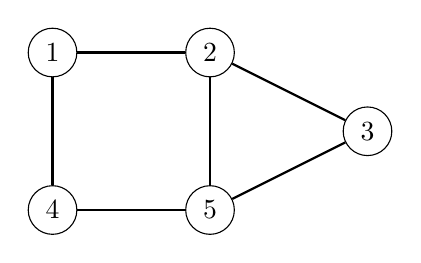
\begin{tikzpicture}
\node[draw, circle] (2) at (5,5) {$2$};
\node[draw, circle] (1) at (3,5) {$1$};
\node[draw, circle] (3) at (7,4) {$3$};
\node[draw, circle] (5) at (5,3) {$5$};
\node[draw, circle] (4) at (3,3) {$4$};

\path[draw,thick,-] (1) -- (2);
\path[draw,thick,-] (2) -- (5);
\path[draw,thick,-] (5) -- (4);
\path[draw,thick,-] (4) -- (1);
\path[draw,thick,-] (2) -- (3);
\path[draw,thick,-] (5) -- (3);
\end{tikzpicture}
\end{center}

これはノード1からの探索が次のようになるので条件を満たしません。
\begin{center}
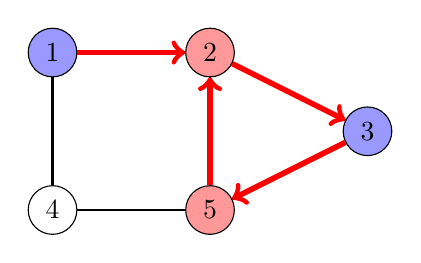
\begin{tikzpicture}
\node[draw, circle,fill=red!40] (2) at (5,5) {$2$};
\node[draw, circle,fill=blue!40] (1) at (3,5) {$1$};
\node[draw, circle,fill=blue!40] (3) at (7,4) {$3$};
\node[draw, circle,fill=red!40] (5) at (5,3) {$5$};
\node[draw, circle] (4) at (3,3) {$4$};

\path[draw,thick,-] (1) -- (2);
\path[draw,thick,-] (2) -- (5);
\path[draw,thick,-] (5) -- (4);
\path[draw,thick,-] (4) -- (1);
\path[draw,thick,-] (2) -- (3);
\path[draw,thick,-] (5) -- (3);

\path[draw=red,thick,->,line width=2pt] (1) -- (2);
\path[draw=red,thick,->,line width=2pt] (2) -- (3);
\path[draw=red,thick,->,line width=2pt] (3) -- (5);
\path[draw=red,thick,->,line width=2pt] (5) -- (2);
\end{tikzpicture}
\end{center}
隣接するノード2と5は共に赤です。したがって、このグラフは二部グラフにはできません。

利用可能な色が2色しかない場合、コンポーネントの開始ノードの色がそのコンポーネントの他のすべてのノードの色を決定します。
開始ノードが赤であろうと青であろうと、結果は変わりません。

ここで注意があります。グラフのノードを$k$色で着色して,隣接するノードが同じ色にならないようにできるかどうかを調べることは非常に困難です。
$k = 3$ の場合でも、効率的なアルゴリズムは知られておらず、この問題は NP困難$(NP-hard)$ です。